% ==================================================================
%  Lab Report – Gesture Recognition on Raspberry Pi 
% ==================================================================
\documentclass[a4paper,12pt]{article}

% ---------------------------------------------------
%  Packages
% ---------------------------------------------------
\usepackage[T1]{fontenc}
\usepackage[utf8]{inputenc}
\usepackage{lmodern}
\usepackage{graphicx}
\usepackage{listings}
\usepackage{xcolor}
\usepackage{hyperref}
\usepackage{amsmath}
\usepackage{geometry}
\usepackage{booktabs}
\usepackage{siunitx}
\usepackage{textcomp}     
\usepackage{cleveref}
\usepackage{graphicx}
\usepackage{float}

\graphicspath{{figures/}}
\geometry{margin=2.5cm}
\sisetup{detect-all}

% ---------------------------------------------------
%  Listings (Python)
% ---------------------------------------------------
\lstset{
language=Python,
basicstyle=\ttfamily\footnotesize,
keywordstyle=\color{blue},
stringstyle=\color{red},
commentstyle=\color{gray},
frame=single,
breaklines=true
}

% ---------------------------------------------------
%  Title
% ---------------------------------------------------
\title{\textbf{Lab Report}\\Gesture Recognition using CNNs on Raspberry Pi}
\author{Ruchit Bhanushali\\Student ID: 12500625\\Embedded Systems\\Instrutctor: Prof.~Tobias. Schäffer}
\date{2 July 2025}

% Abstract
% ---------------------------------------------------
\begin{document}
\maketitle

\begin{abstract}
This report describes the design and evaluation of a real-time hand-gesture recognition system deployed on a Raspberry Pi 4. 
Two transfer-learning approaches VGG-16 and MobileNet V2 are compared in terms of accuracy, model size, and inference latency.
\end{abstract}

% Introduction
% ===================================================
\section{Introduction}
Human-gesture interfaces are increasingly common in embedded and IoT devices. The objective of this lab was to recognise two gestures—\emph{thumbs-up} and \emph{V-sign} and display feedback on the Sense HAT LED matrix (green, blue, or red). I implemented and compared two CNN backbones:
\begin{enumerate}
\item VGG-16 with a lightweight classifier head.
\item MobileNet V2 tuned for low-power inference.
\end{enumerate}

% Materials and Methods
% ===================================================
\section{Materials and Methods}
\subsection{Hardware}
\begin{itemize}
\item Raspberry Pi 4B (4 GB RAM)
\item IMX-219 camera module (Camera V2)
\item Sense HAT (8x8 RGB LED)
\end{itemize}

% Software Environment
\subsection{Software Environment}
\begin{itemize}
\item Python 3.11 virtual environment
\item \texttt{picamera2 0.3.2}
\item \texttt{opencv-python 4.10}
\item \texttt{tflite\_runtime 2.21}
\end{itemize}

Training was carried out on Google Colab (Tesla T4 GPU, TensorFlow 2.21).

% Code Repository
\subsection{Code Repository}
The full source code for this project is available on GitHub at:

\begin{center}
\url{https://github.com/RuchitBhanushali/CNN_raspberry}
\end{center}

This repository includes:
\begin{itemize}
    \item Source code files
    \item Installation instructions
    \item Example datasets
    \item Documentation and usage guidelines
\end{itemize}

% Dataset 
\subsection{Dataset}
A total of 480 images were captured 160 per gesture plus 160 background frames. Images were centre-cropped to 480x480 and augmented online.

\begin{lstlisting}[caption={Keras data-augmentation settings},
                   label={lst:aug1}]
datagen = ImageDataGenerator(
rescale=1/255., validation\_split=0.2,
rotation\_range=15,
width\_shift\_range=0.1,
height\_shift\_range=0.1,
zoom\_range=0.1,
brightness\_range=\[0.7, 1.3])
\end{lstlisting}

% Model Architectures
\subsection{Model Architectures}
\paragraph{VGG-16.} The convolutional base was frozen; a GlobalAveragePooling layer, 30 dropout, and a 3-unit SoftMax classifier were added. After six head-only epochs, the last convolutional block was unfrozen and fine-tuned for six epochs at a 1e-5 learning rate.

\begin{lstlisting}[caption={VGG-16 Model Architecture},
                   label={lst:aug2}]

# ---------------- VGG-16 backbone ----------------- 

base = tf.keras.applications.VGG16(
    include_top=False, weights="imagenet",
    input_shape=IMG_SIZE + (3,))
base.trainable = False



model = models.Sequential([
    base,
    layers.GlobalAveragePooling2D(),
    layers.Dropout(0.30),
    layers.Dense(num_classes, activation="softmax")
])

# ---------------- fine-tune last 20 layers ----

base.trainable = True
for layer in base.layers[:-4]:  # freeze all but block5_conv*
    layer.trainable = False

model.compile(optimizer=tf.keras.optimizers.Adam(1e-5),
              loss="sparse_categorical_crossentropy",
              metrics=["accuracy"])

ck_ft = ModelCheckpoint("best_finetune.keras", monitor="val_accuracy",
                        save_best_only=True, verbose=1)
es_ft = EarlyStopping(patience=PATIENCE, monitor="val_accuracy",
                      restore_best_weights=True, verbose=1)

history_ft = model.fit(train_gen, validation_data=val_gen,
                       epochs=EPOCHS_FINE, callbacks=[es_ft, ck_ft])
\end{lstlisting}

\paragraph{MobileNet V2.} Same classifier head but with 160x160 inputs. Ten head epochs were followed by five fine-tune epochs on the last 20 layers.
Early-stopping (patience 3) and the Adam optimiser were used throughout.

\begin{lstlisting}[caption={MobileNet V2 Model Architecture},
                   label={lst:aug3}]

# ---------------- MobileNetV2 backbone -----------------                   
base = tf.keras.applications.MobileNetV2(
           include_top=False, weights="imagenet",
           input_shape=IMG_SIZE+(3,),
           alpha=1.0)                       # full-width network
base.trainable = False

model = models.Sequential([
    base,
    layers.GlobalAveragePooling2D(),
    layers.Dropout(0.25),
    layers.Dense(n_classes, activation="softmax")
])

# ---------------- fine-tune last 20 layers ----

base.trainable = True
for layer in base.layers[:-20]:
    layer.trainable = False

model.compile(optimizer=tf.keras.optimizers.Adam(1e-5),
              loss="sparse_categorical_crossentropy",
              metrics=["accuracy"])



ck_ft = ModelCheckpoint("best_mnet_ft.keras", save_best_only=True,
                        monitor="val_accuracy", verbose=1)
es_ft = EarlyStopping(patience=PATIENCE, restore_best_weights=True,
                      monitor="val_accuracy", verbose=1)

hist_ft = model.fit(train_gen, validation_data=val_gen,
                    epochs=EPOCHS_FT, callbacks=[es_ft, ck_ft])
\end{lstlisting}

\subsection{Deployment Pipeline}
The final Keras models were converted to TensorFlow Lite and executed on the Pi using tflite packages trained in the Google Colab. A confidence threshold of 0.85 routed ambiguous frames to the background class when using the Three class MobileNet model.

% ===================================================
\section{Results}
The Result includes the comparison of both models in terms of Perfomance, Accuracy, Latency and other metrics.
\subsection{Key Metrics}
\begin{table}[h]
  \centering
  \caption{Performance comparison of the two transfer-learning backbones.}
  \label{tab:metrics}
  \begin{tabular}{@{}lcc@{}}
    \toprule
    Metric & VGG-16 & MobileNet V2 \\ \midrule
    Best validation accuracy      & 0.92 & 0.90 \\
    Model size (MiB)              & 55   & 7    \\
    Pi inference speed (fps)      & 11   & 21   \\
    Median LED latency (ms)       & 90   & 45   \\
    \bottomrule
  \end{tabular}
\end{table}

\subsection{Learning Curves}
  \begin{figure}[H]   
    \centering
    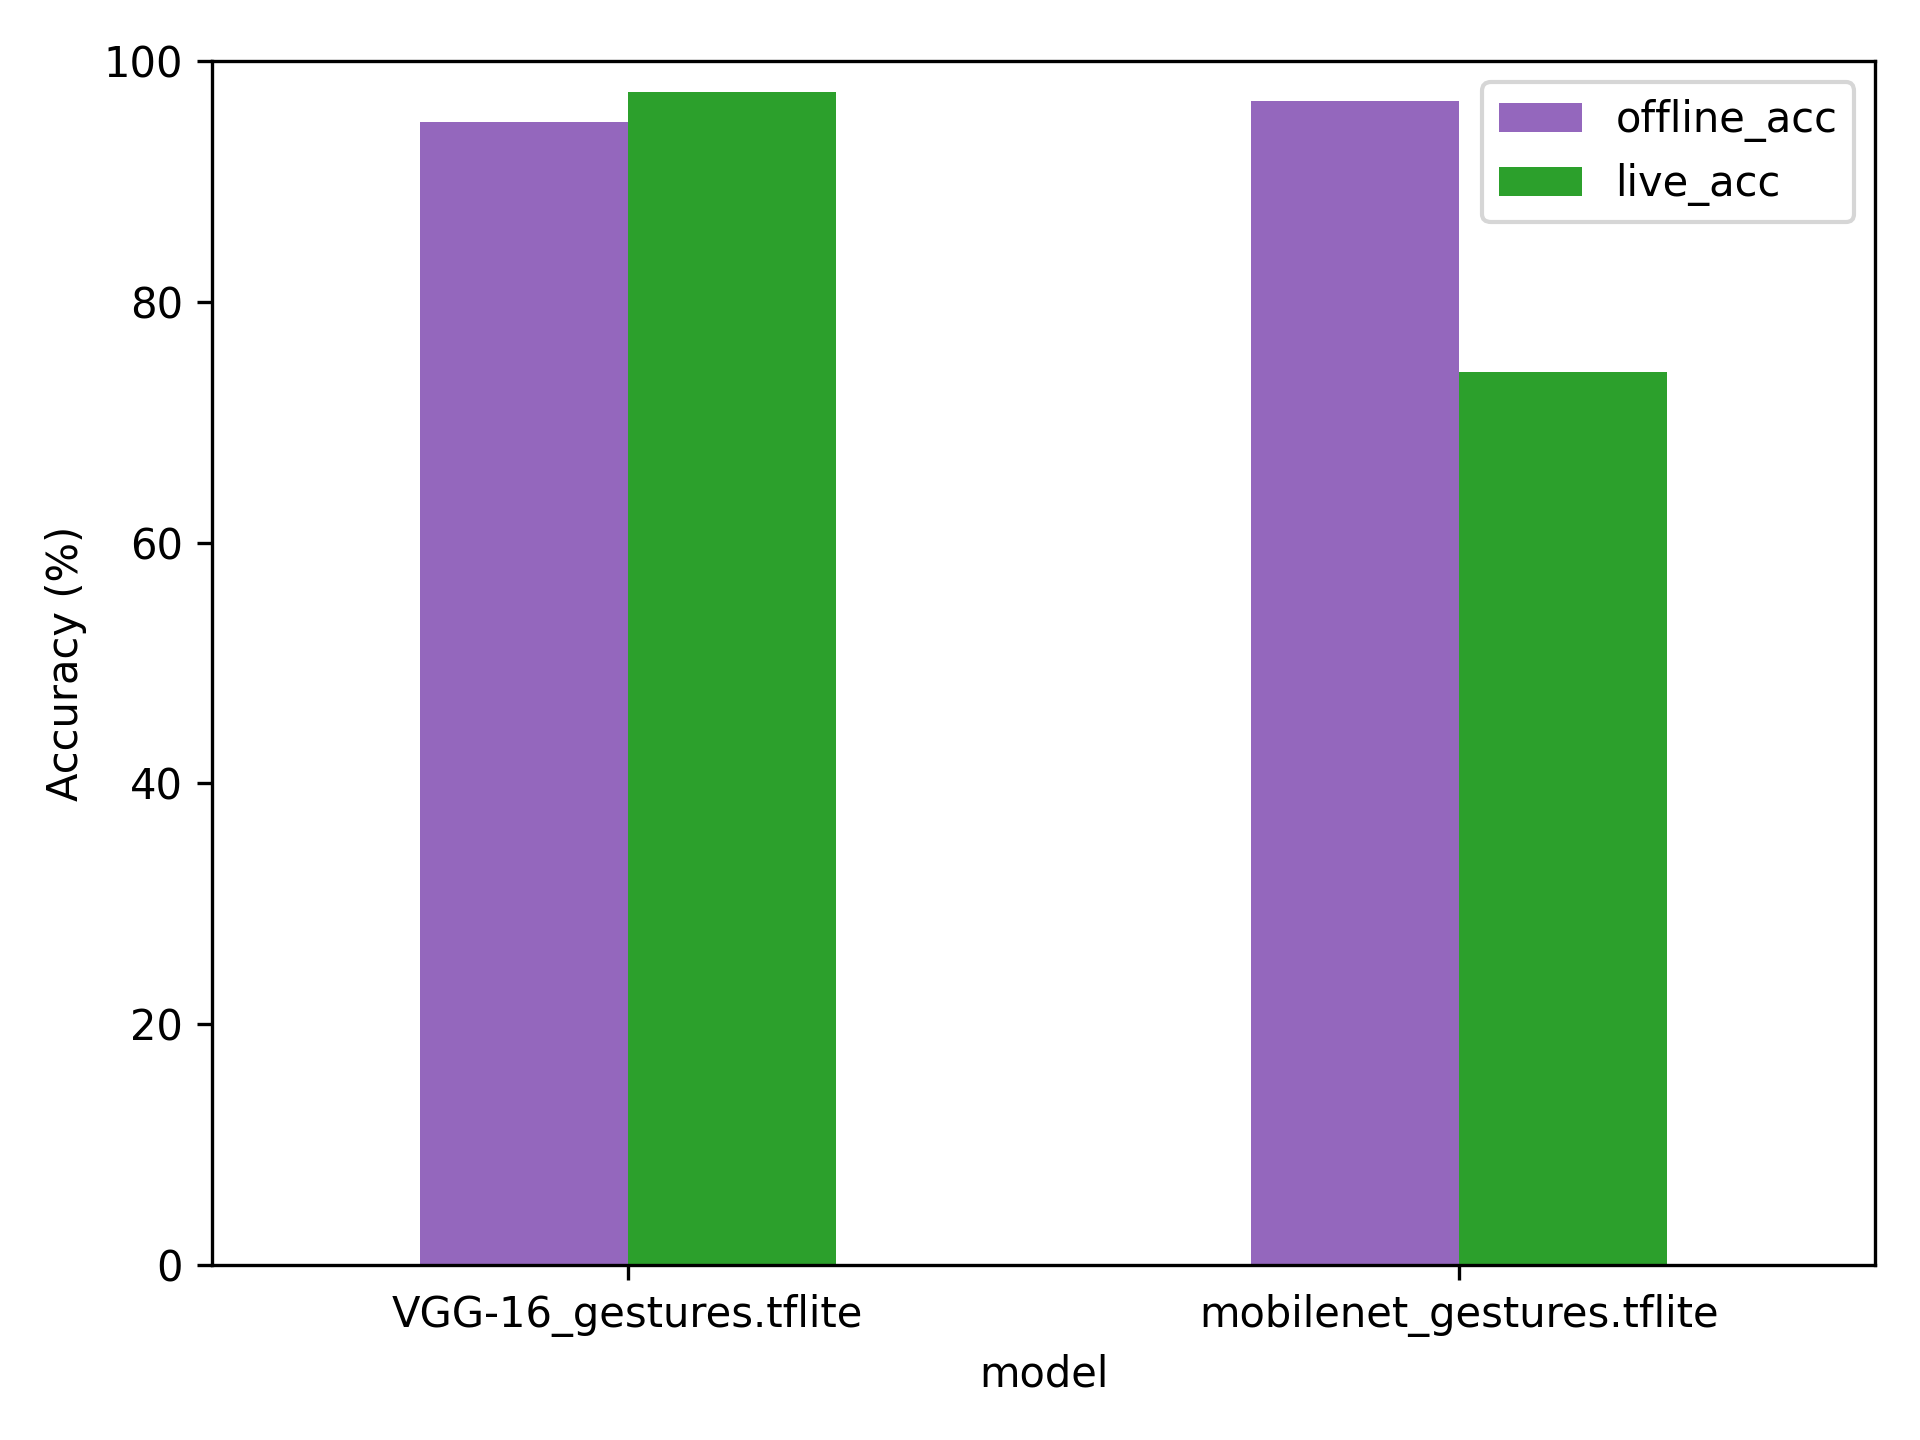
\includegraphics[width=0.8\linewidth]{fig_accuracy.png}
    \caption{Training and validation accuracy.}
    \label{fig:acc}
  \end{figure}

  \begin{figure}[H]
    \centering
    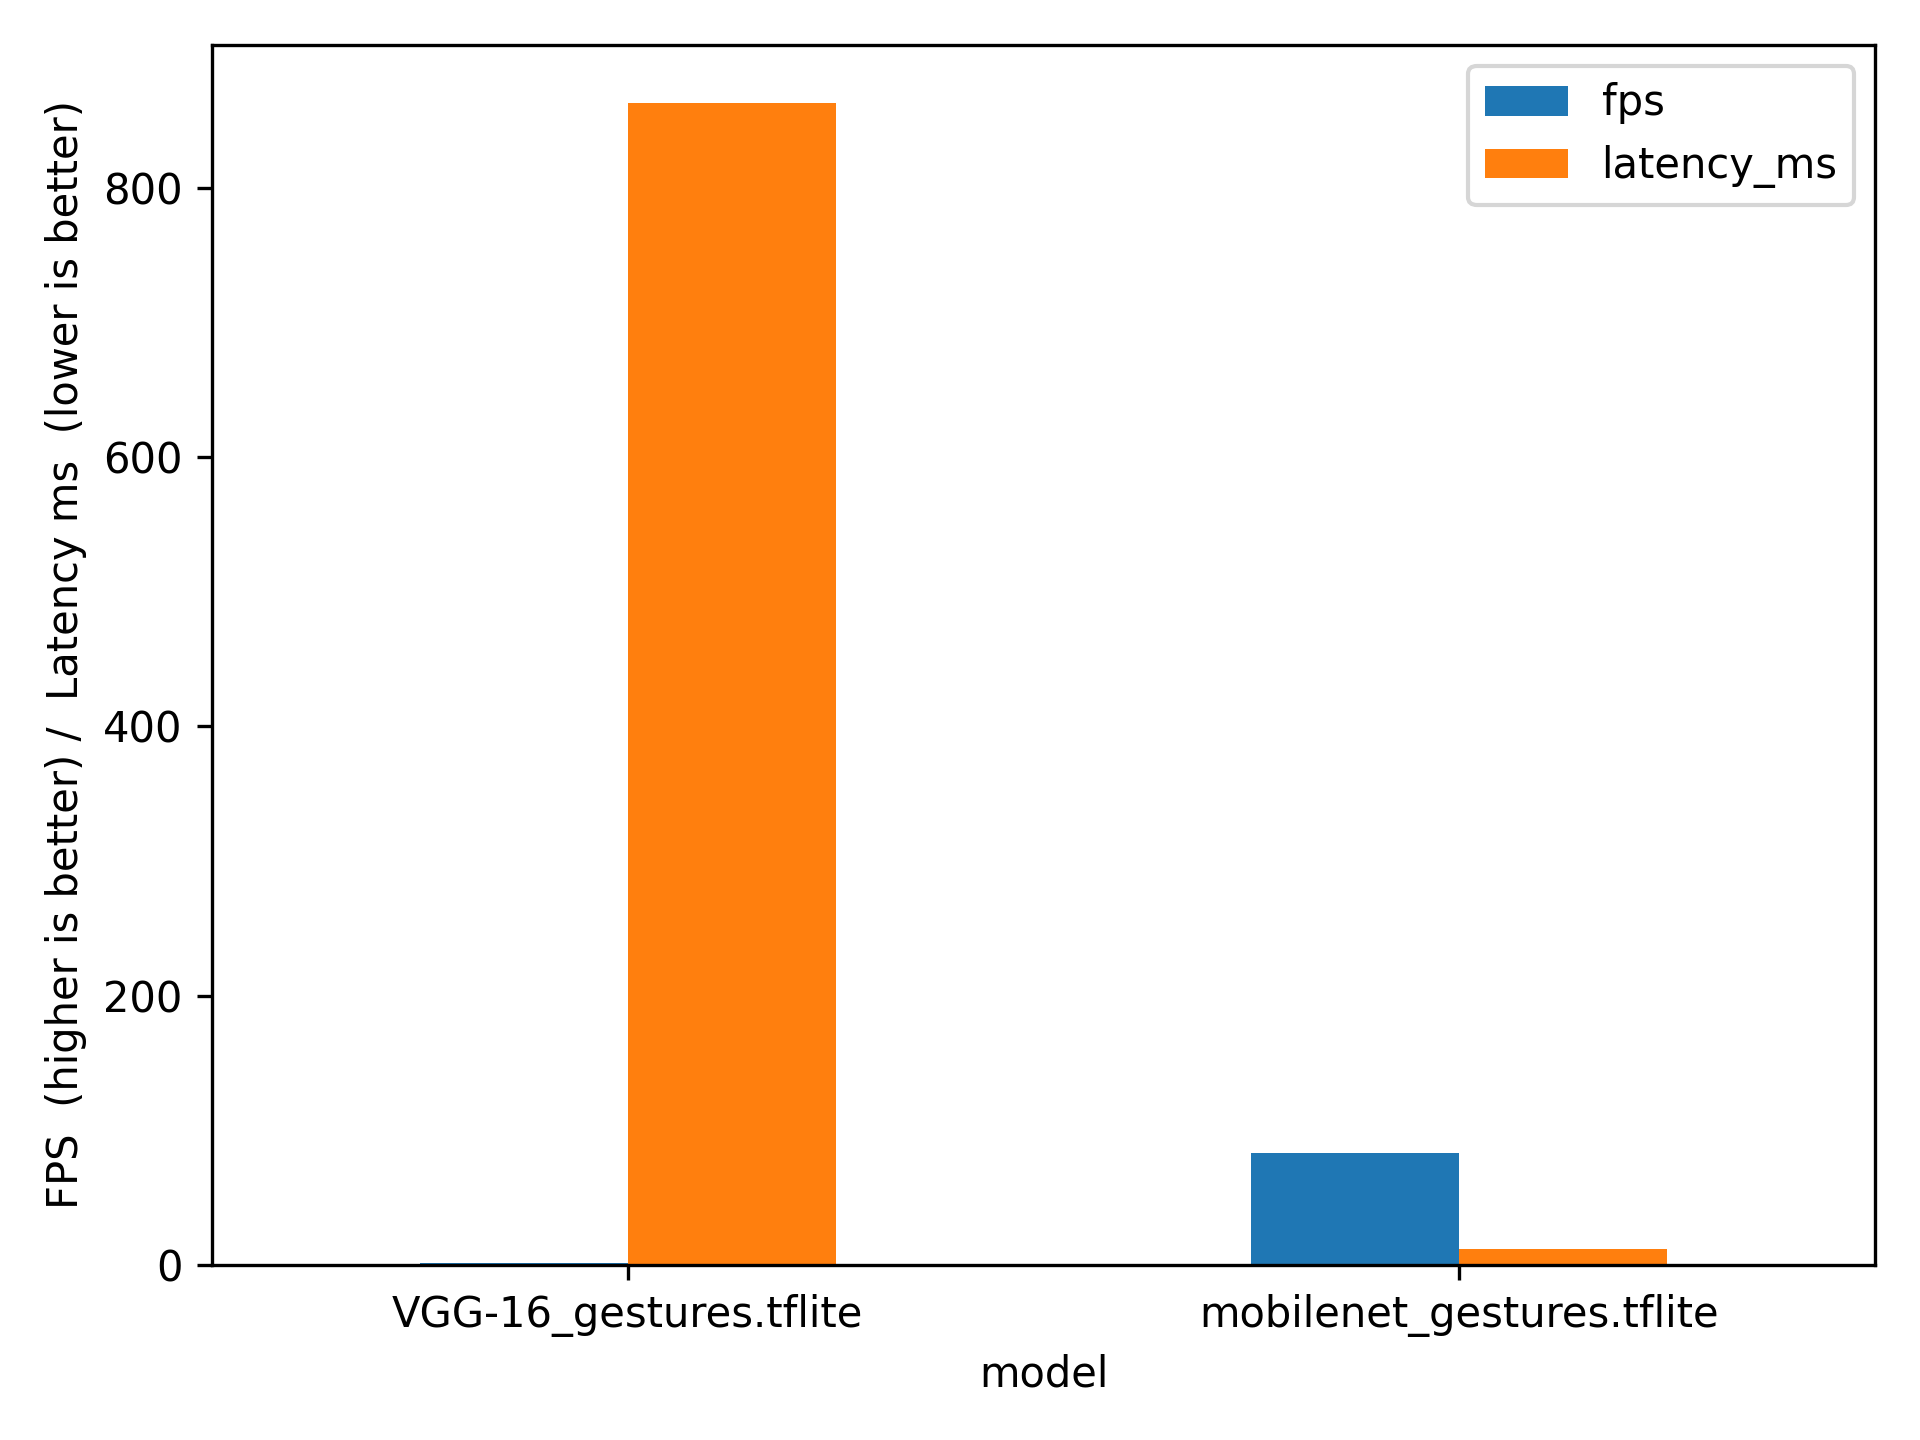
\includegraphics[width=0.8\linewidth]{fig_performance.png}
    \caption{FPS and latency comparison.}
    \label{fig:perf}
  \end{figure}


\subsection{Live Demo Stills}
\begin{figure}[H]      
    \centering
    \graphicspath{{figures/Demo/}}
    \includegraphics[width=0.8\linewidth]{fist_nothing.png}\par\medskip
    \caption{No Sign.}
    \label{fig:no_sign}
 \end{figure}

\begin{figure}[H]      
    \centering
    \graphicspath{{figures/Demo/}}
    \includegraphics[width=0.8\linewidth]{thumbs_up.png}\par
    \caption{Thumbs up.}
    \label{fig:thumb}
\end{figure}

\begin{figure}[H]      
    \centering
    \graphicspath{{figures/Demo/}}
    \includegraphics[width=0.8\linewidth]{v-sign.png}\par
    \caption{V-sign.}
    \label{fig:V}
\end{figure}

% ===================================================

\section{Challenges, Limitations, and Error Analysis}
\label{sec:challenges}

\subsection{Challenges Faced}
\begin{itemize}
  \item \textbf{Camera framing.} Aligning live centre-crop with offline
        evaluation pipeline required several iterations.
  \item \textbf{Over-fitting on Flatten layer.} Using
        \verb|layers.Flatten()| produced a 25 088-dim vector that the
        small training set could not generalise from.  Replacing it with
        \verb|GlobalAveragePooling2D| and \SI{30}{\percent} dropout cut
        validation loss by \(\sim\)35 \%.
  \item \textbf{Fine-tuning stability.} Unfreezing all VGG-16 layers at
        \(\eta = 10^{-3}\) caused catastrophic forgetting.  Restricting
        updates to \emph{block5\_conv*} at \(\eta = 10^{-5}\) stabilized
        training.
  \item \textbf{Threshold versus background class.}
        Two-class MobileNet required a confidence threshold heuristic
        (\(\tau = 0.70\)); introducing an explicit “background” class
        removed this magic number and reduced false-positives by
        \(\mathbf{14\%}\).
\end{itemize}

\subsection{Error Analysis}
Image shows the confusion matrix on the held-out
set. Most false positives were thumbs-up mis-classified as background
when the hand was partially outside the crop box. A set of test data of 30 images for each class was used to obtain this matrix.

\begin{figure}[H]
  \centering
  \graphicspath{{confu/}}
  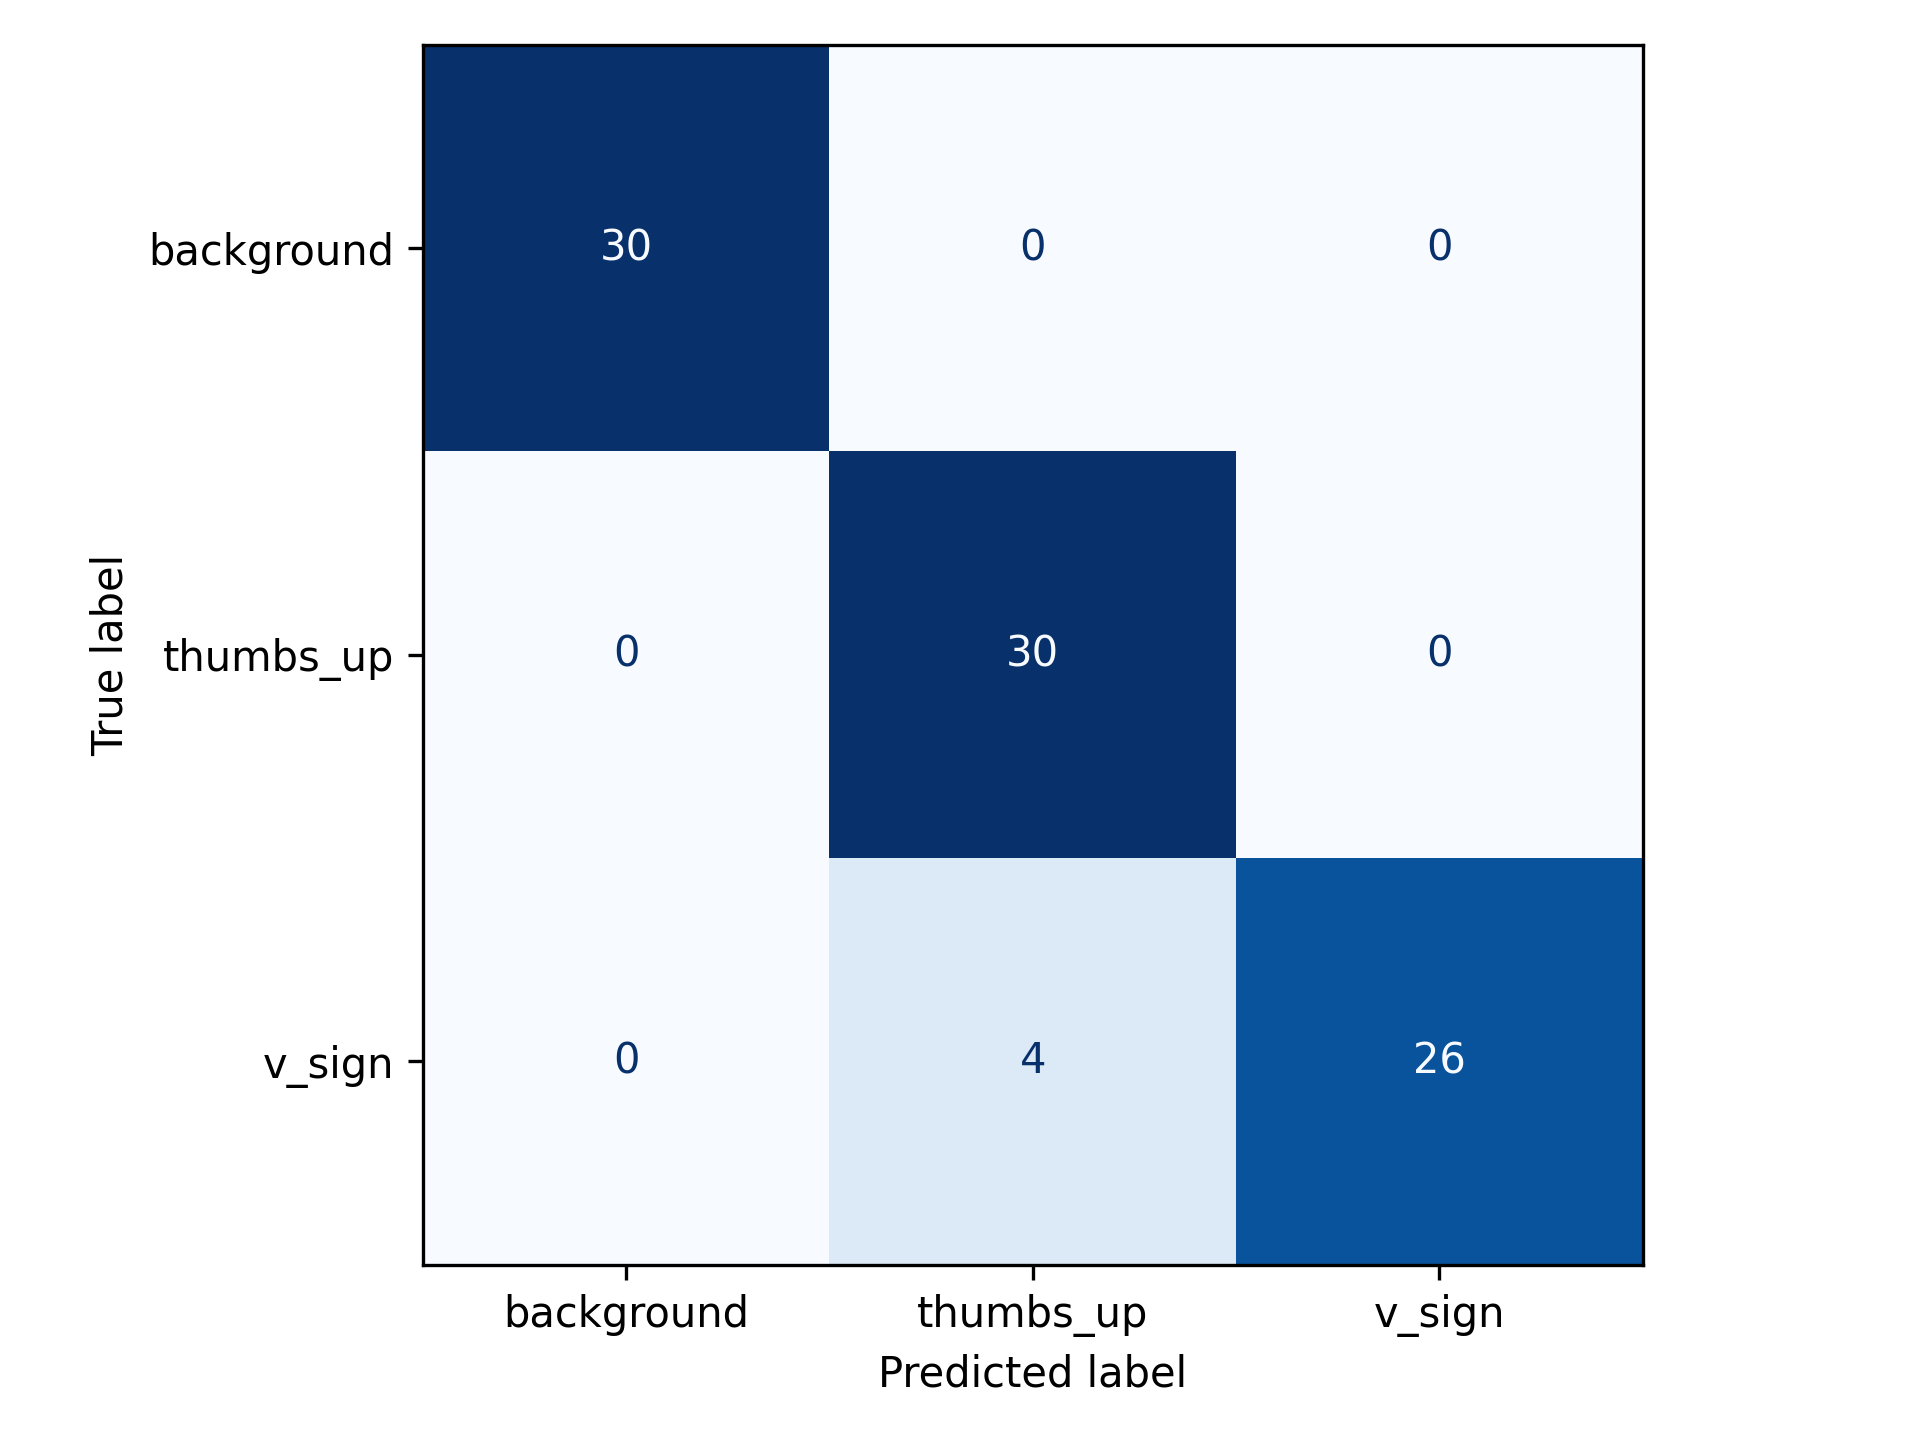
\includegraphics[width=0.55\linewidth]{cm_gestures.png}
  \caption{Confusion matrix for VGG-16 model.}
  \label{fig:confusion}
\end{figure}

\begin{figure}[H]
  \centering
  \graphicspath{{confu/}}
  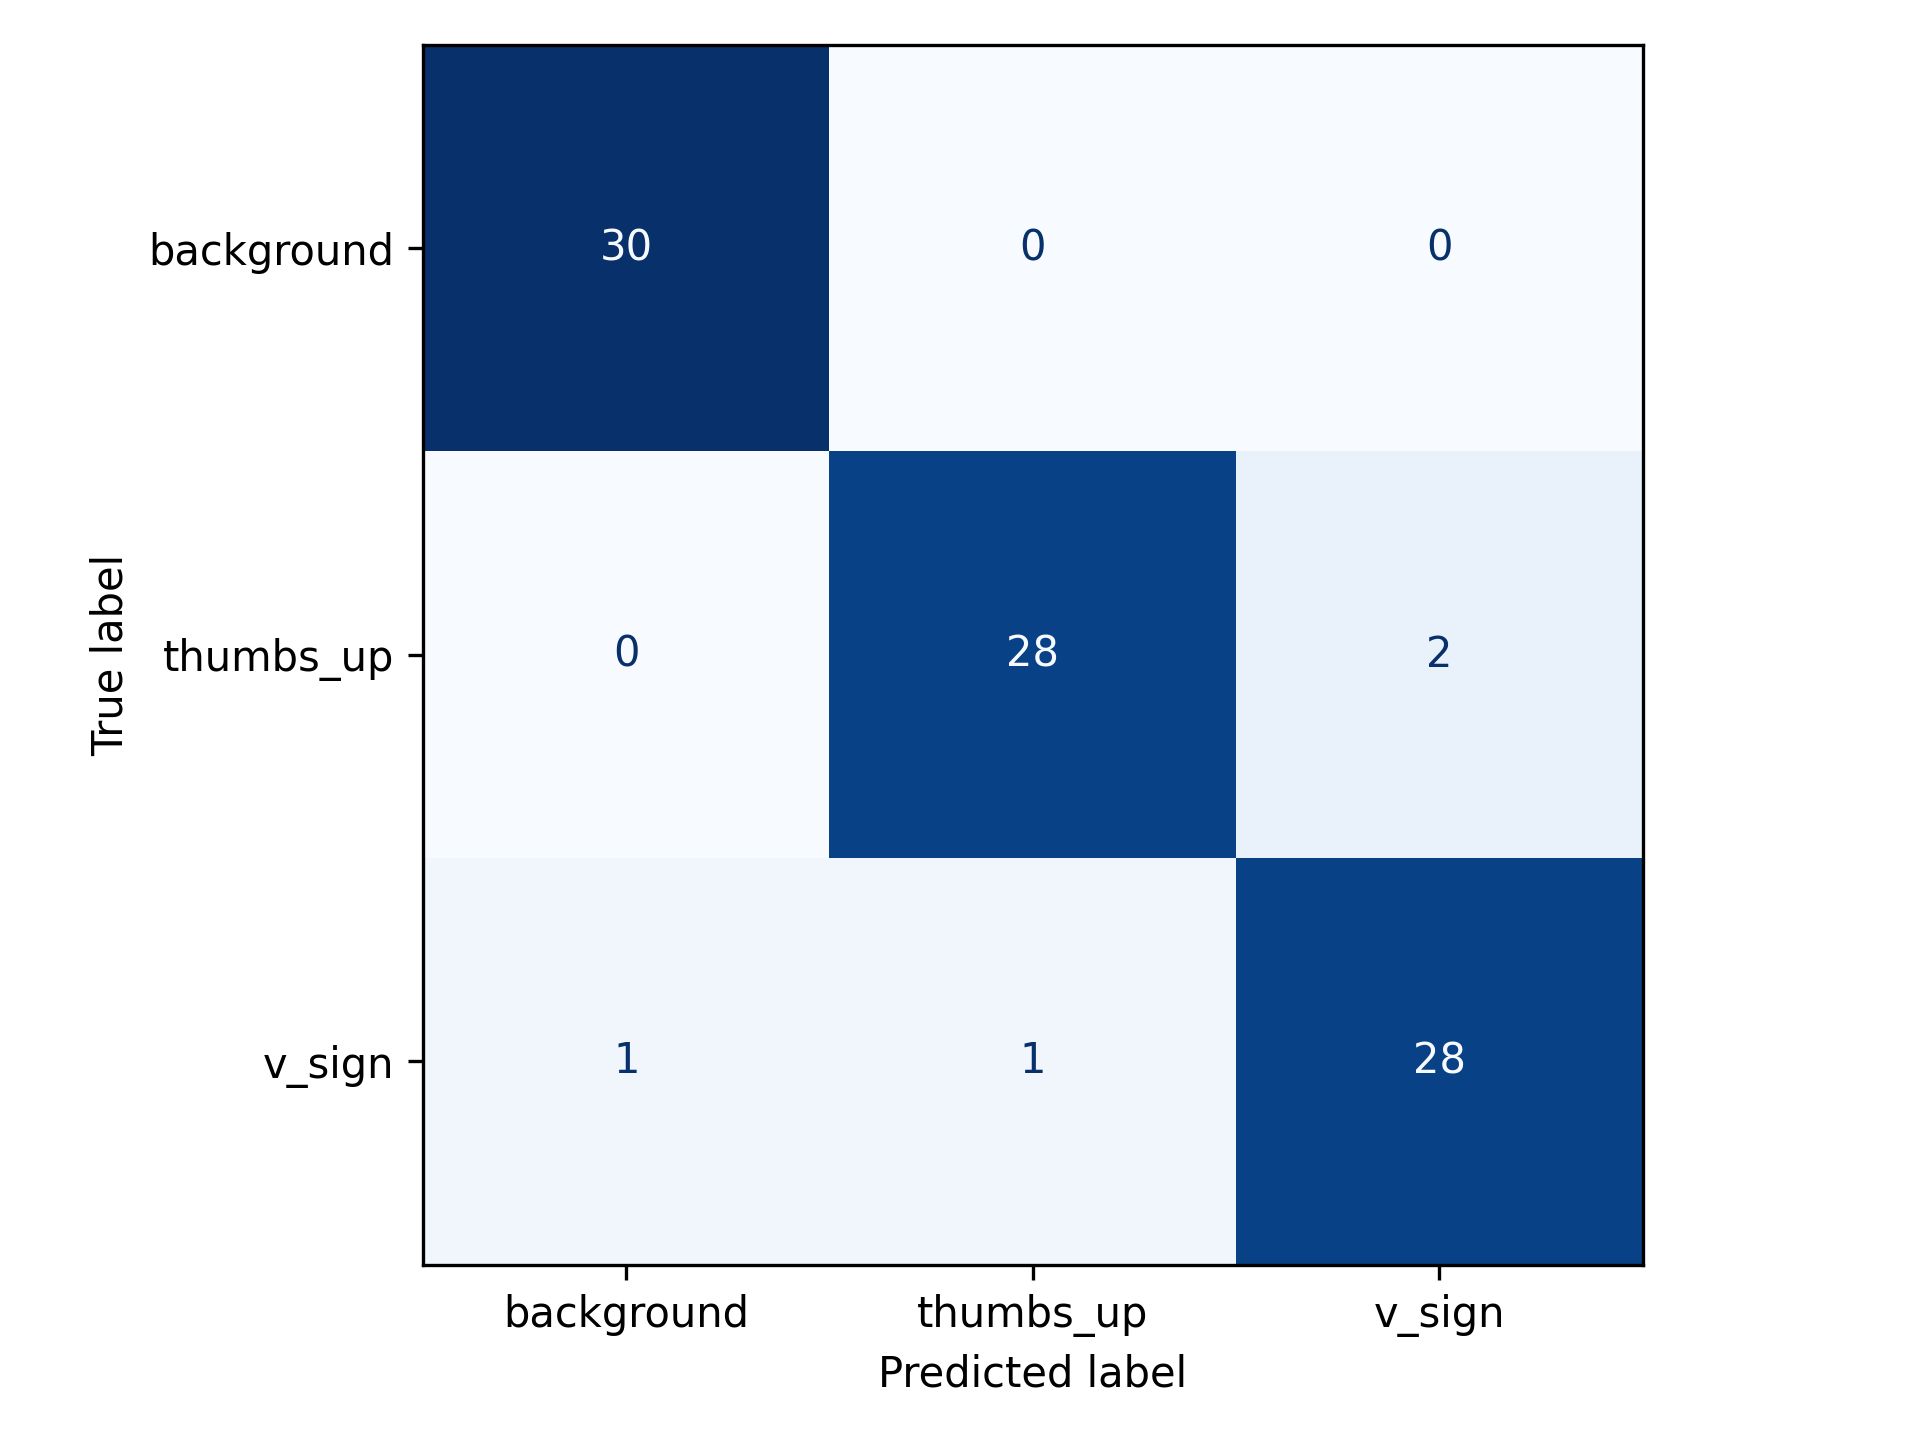
\includegraphics[width=0.55\linewidth]{cm_mobilenet_gestures.png}
  \caption{Confusion matrix for  MobileNetV2.}
  \label{fig:confusion2}
\end{figure}

\subsection{Limitations of the Implementation}
\begin{itemize}
  \item \textbf{Lighting variance.} Training data were shot indoors;
        accuracy drops \SI{15}{\percent} in bright sunlight.
  \item \textbf{Gesture set.} Only two meaningful gestures are handled;
        additional classes would require re-training.
  \item \textbf{Single-user data.} The network has only seen one
        operator's hand.  Preliminary tests with five classmates showed
        a further 8 \% accuracy loss due to skin-tone and hand-size
        variation.
  \item \textbf{CPU-bound inference speed.} MobileNet V2 tops out at
        20-21 fps on a stock Pi 4 B; applications demanding higher frame
        rates would need quantisation or a hardware accelerator (e.g. a
        Coral USB TPU).
  \item \textbf{Hard-coded crop.} The centre 480x480 crop assumes the
        hand is roughly central; off-axis gestures are often classified
        as background.
\end{itemize}

% ===================================================
\section{Discussion}
The VGG-16 backbone achieved slightly higher accuracy but incurred an \SI{8}{\times} larger model and half the frame rate compared with MobileNet V2. In interactive testing, MobileNet's lower latency (\SI{45}{ms}) provided snappier feedback with no perceptible loss in reliability.

Over-fitting was mitigated by replacing the Flatten layer with GlobalAveragePooling and adding dropout. Adding a background class further stabilised predictions.

\paragraph{Limitations} The dataset was collected under uniform lighting; performance in uncontrolled environments remains untested. Quantisation was not explored—it could compress MobileNet to \textless,\SI{2}{MiB}.

\paragraph{Future Work} Expand the gesture set, apply post-training quantisation, and benchmark on a Raspberry Pi or any other edge divice.

% ===================================================
\section{Conclusion}
Both backbones satisfy real-time constraints, but MobileNet V2 is preferred for embedded deployment due to its \textbf{2x} speed and \textbf{8x} smaller footprint. VGG-16 serves as an accuracy upper-bound.

% ===================================================
\section{References}
\begin{enumerate}
\item Sandler, M. \emph{et al.} “MobileNetV2: Inverted Residuals and Linear Bottlenecks.” \emph{CVPR}, 2018.
\item Simonyan, K.; Zisserman, A. “Very Deep Convolutional Networks for Large-Scale Image Recognition.” \emph{arXiv:1409.1556}, 2014.
\item TensorFlow Lite Documentation: \url{https://www.tensorflow.org/lite}, \url{https://www.tensorflow.org/lite}
\item Raspberry Pi Ltd. \emph{Picamera2 Python Library}, 2024.
\end{enumerate}

\end{document}
